Before one can understand what exactly is behind the term "rhythm game", one needs to understand the history and heritage of the genre. The first game to introduce gameplay that somehow resembles part of the mechanics of contemporary rhythm games is \textit{Simon}, created in 1978 by Ralph Baer and Howard Morrison. In this handheld electronic game, the player needs to repeat the sequence in which the buttons light up. The sequence becomes progressively longer, up to the point when a player is unable to repeat it in the right order. There was no background music to speak of, so it cannot be considered a fully-fledged rhythm game, but the action of repeating sequences and patterns is a fundamental part of present-day rhythm games genre.

\begin{figure}[h]
    \centering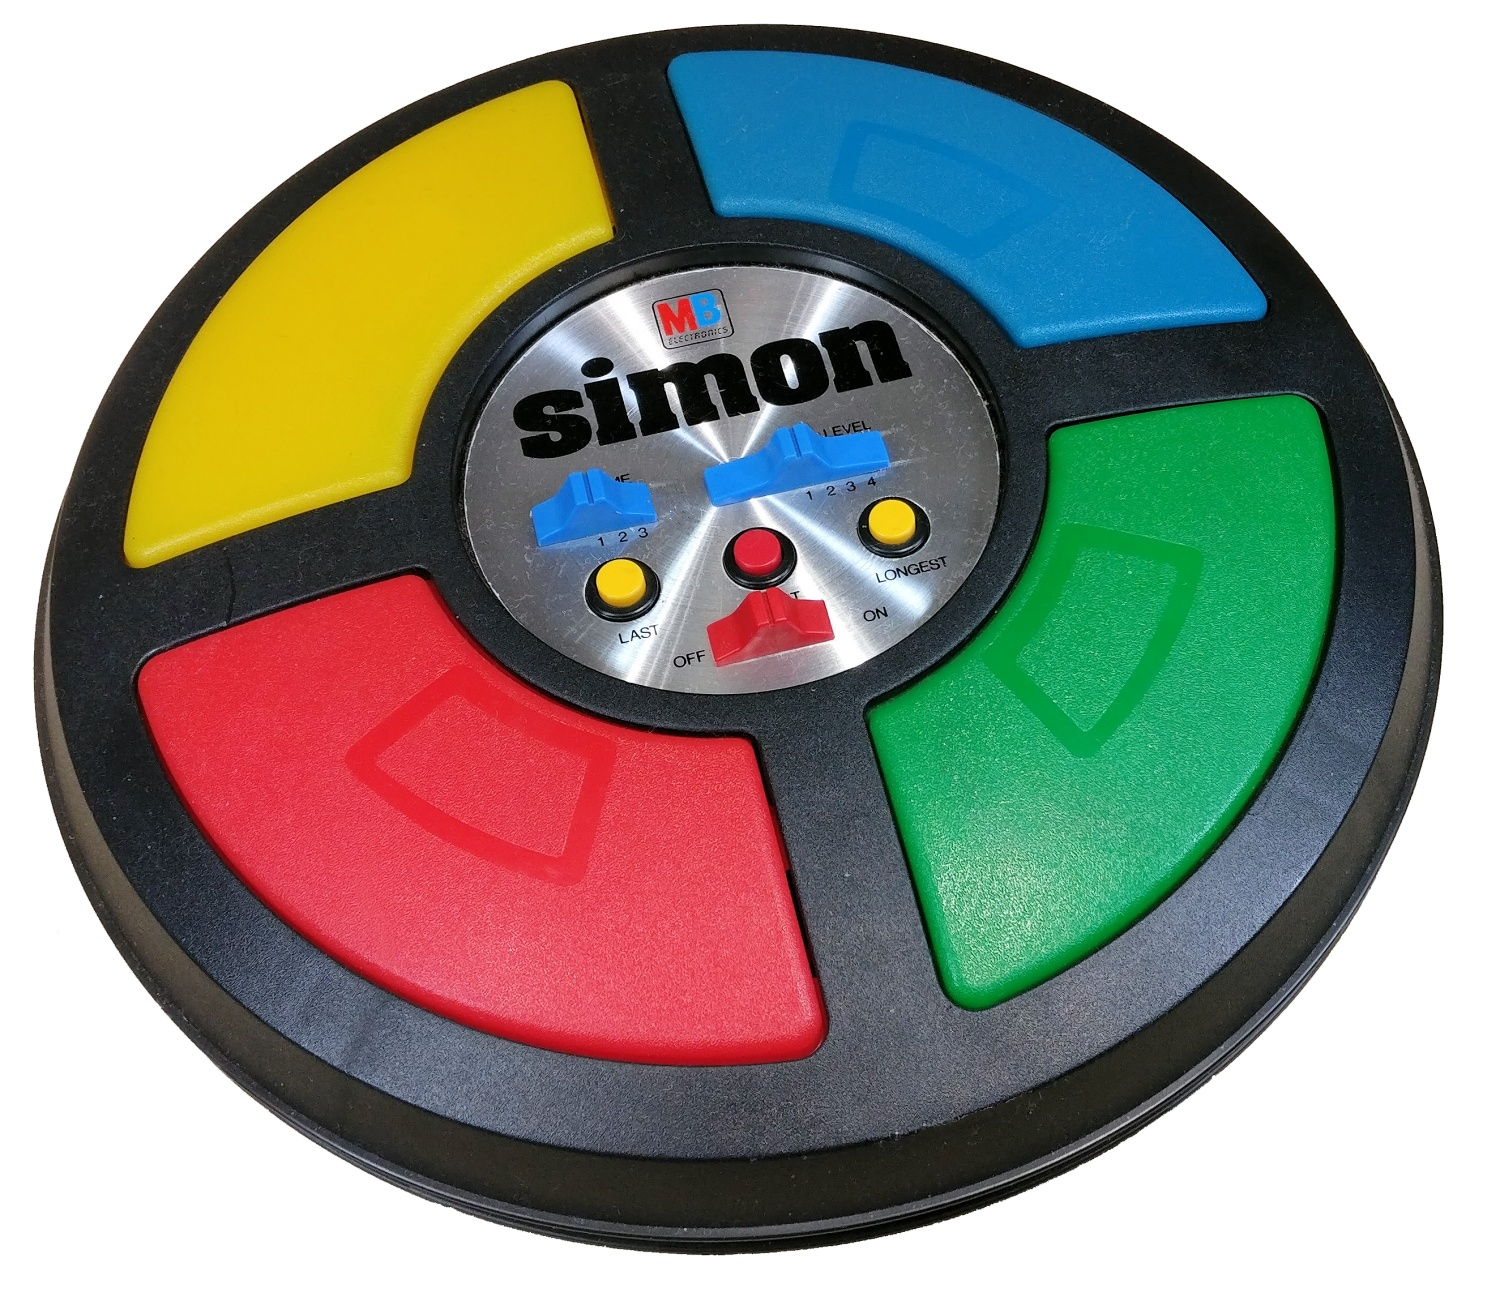
\includegraphics[scale=0.05]{obrazki/simon.jpg}
    \caption{Electronic game \textit{Simon} - It became a massive worldwide success, becoming a pop culture symbol. The game spawned many different releases and imitators with similar or same basic gameplay. \cite{simongame}}
    \label{fig:simon_game}
\end{figure}

The first rhythm game that can be recognized as such is \textit{PaRappa the Rapper} (1996), published by Sony Computer Entertainment for the PlayStation platform, building its core gameplay around music. Because of its unique art style, good narrative, and catchy soundtrack, the game was well received among players and critics, being listed as one of the best video games ever made several times. \cite{acclaimed_videogames_parappa} This success contributed significantly to the rise in popularity of the genre. In \textit{PaRappa the Rapper}'s gameplay, the player must press correct buttons in response to the rhythm of the currently playing track and symbols that appear on the top of the screen. This mechanic of pressing the corresponding buttons will be further described as "hit". The correct sequence is first performed by a teacher, after which PaRappa needs to respond accordingly. Pressing the correct buttons in accordance with the rhythm results in PaRappa rapping. One can observe the resemblance to the aforementioned \textit{Simon} electronic game - PaRappa built upon this mechanic, adding additional visual and auditory feedback, background music and grading system, setting the stage for further developments of this genre. Especially important was the addition of background music synced with other gameplay elements, making it easier to time the hits correctly. The player's final accuracy is graded from Awful to Cool -- this is currently a standard, expected element of every representative of the genre. The score is affected not only by omitted hits but also by less-than-ideal hits -- the more accurate the hit, the better the rating. As Melanie Fritsch describes in \textit{History of Video Game Music} \cite{MusicMedien}: "The player had to repeat a sequence of sounds, not only by getting the correct sequence (by hitting the correct buttons), but also by the timing of the sequence. Points were given for correctness as well as for “style”. For a higher rating, the player had to “freestyle”, which meant varying from the given sequence but still keeping in time with the song’s rhythm" (Fritsch 2013: 28).

\begin{figure}[h]
    \centering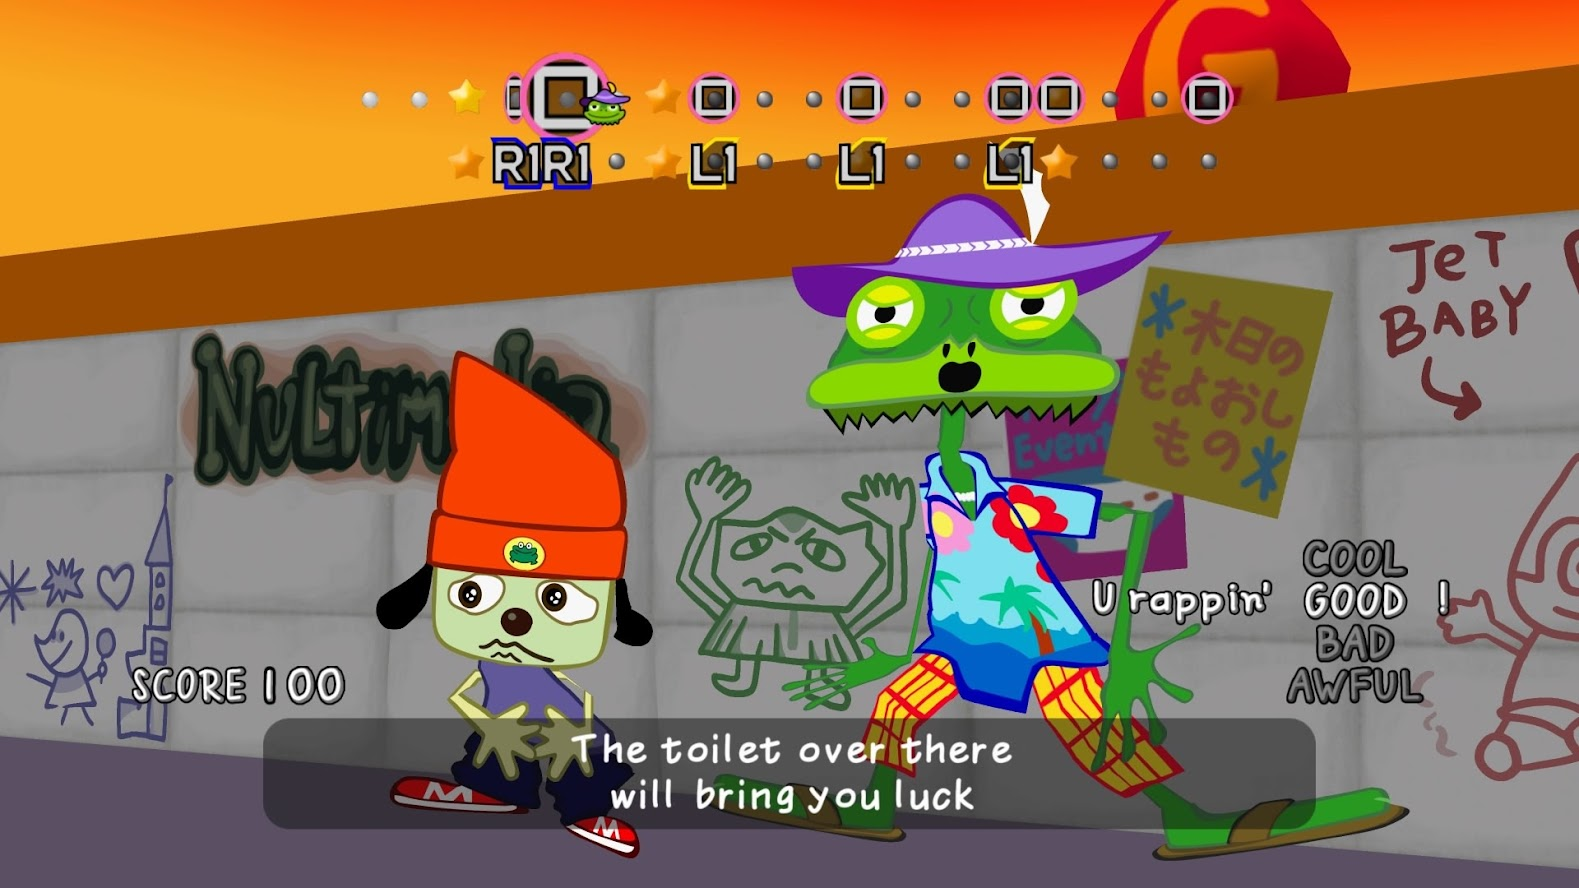
\includegraphics[scale=0.15]{obrazki/parappatherapper.jpg}
    \caption{A frame from \textit{PaRappa the Rapper Remastered} from 2017 showing the input guide at the top of the screen, grading and scoring system. Remastered was used here as an example, but the original had the exact same mechanics back in 1996. \cite{parappatherapper}}
    \label{fig:parappa_the_rapper}
\end{figure}

The release of \textit{beatmania} in 1997 by Konami was another milestone in the development of the rhythm games genre. To enhance the player's experience with a more immersive input device, the game was introduced to Japanese arcades instead of being released on home platforms. \textit{Beatmania}'s arcade cabinet includes a special input device which resembles a DJ console -- it consists of 5 buttons arranged in a piano-like pattern and a round pad that mimics a vinyl record.

\begin{figure}[h]
    \centering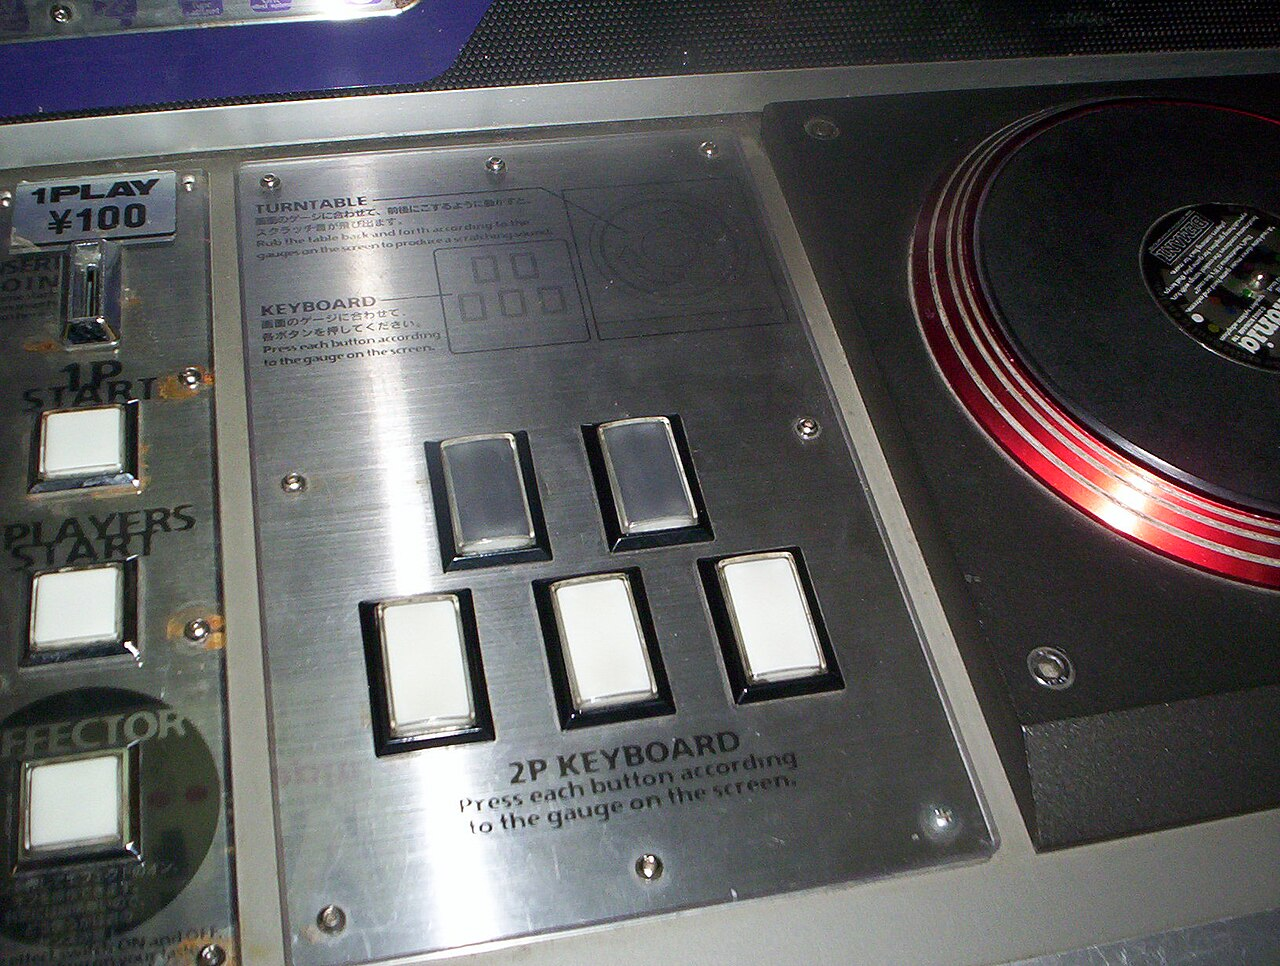
\includegraphics[scale=0.15]{obrazki/beatmaniacontrols.jpg}
    \caption{A controller of 1st \textit{beatmania} arcade release, showing the buttons layout and the turntable. \cite{beatmaniacontrols}}
    \label{fig:beatmania_controls}
\end{figure}

The gameplay is enclosed on a stage that consists of a vertically-scrolling panel with hit-notes on the sides, music video and audience bar in the middle. The player is supposed to press the buttons and turn the turntable in accordance with the notes that are falling from the top to the bottom of the screen, indicating the time to react when they fall down on the judgment line above the illustration of the controller. This is currently known as a vertical scrolling rhythm game -- which \textit{PaRappa the Rapper} could not be considered as such because it showed the input sequences in batches. The game turned out to be a big hit, resulting in Konami putting more effort and resources into Konami's Games and Music Division. Due to the popularity of \textit{beatmania}, this department changed its name to Bemani: "The game was such a huge success that the Games \& Music Division
of the company changed its name to Bemani, which produced and still produces a
long list of spin-offs and sequels" (Fritsch 2013: 28). \cite{MusicMedien} After experimenting with more concepts of rhythm games, they came up with another big hit, which was \textit{Dance Dance Revolution} (1998) -- a pioneering title in the rhythm game genre. It adapted the basic concept of vertical scrolling rhythm game to a new form of input. The game is controlled through a dance platform, with the player standing in the middle and pressing the buttons with their feet.

The core gameplay is very akin to \textit{beatmania}, sans the turntable. The Vertical Scrolling Rhythm Game (VSRG) formula has been adapted to a new type of play with the player in standing position, dancing to the upcoming rhythm notes. This small change resulted in an experience unlike anything before, as following the patterns became even more natural and dancing became a natural result of playing the game properly. The game became an even bigger success than \textit{beatmania}, achieving worldwide popularity, being an introduction to the rhythm game genre for many players around the world. A major factor in this was definitely the natural connection between its input method and gameplay revolving around dancing.

\begin{figure}[h]
    \centering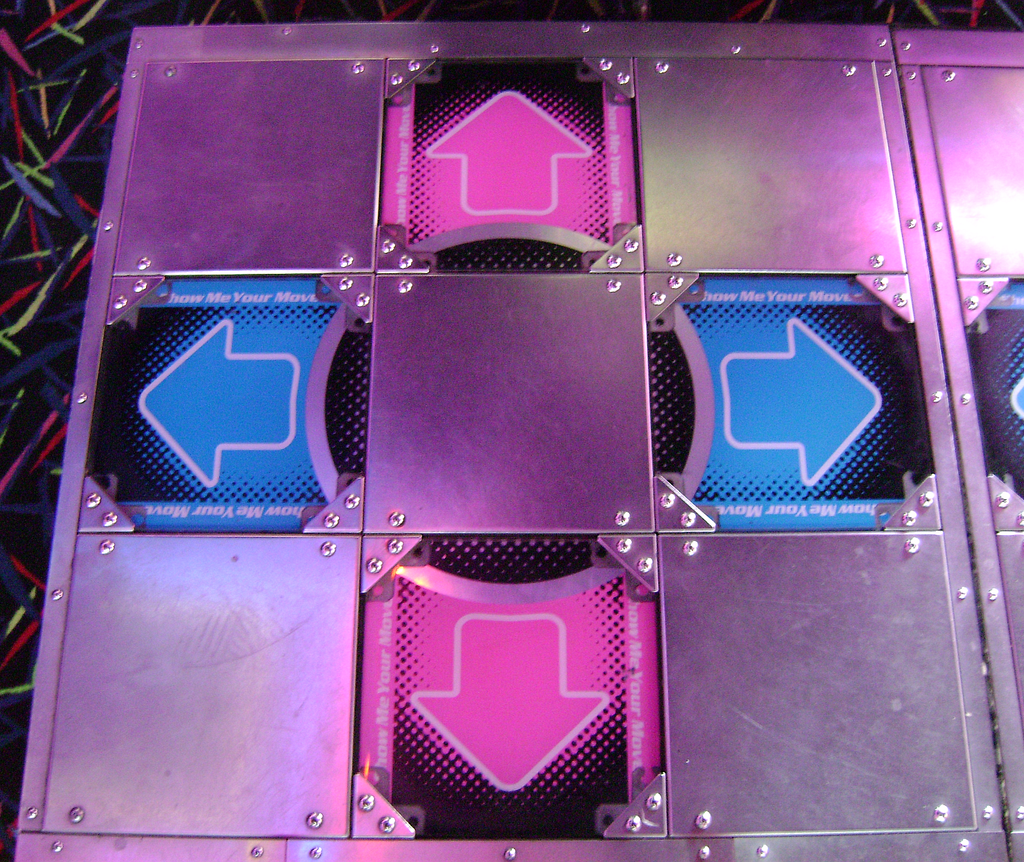
\includegraphics[scale=0.2]{obrazki/ddrplatform.png}
    \caption{A \textit{Dance Dance Revolution} dance platform. \cite{ddrplatform}}
    \label{fig:ddr_platform}
\end{figure}

\begin{figure}[h]
    \centering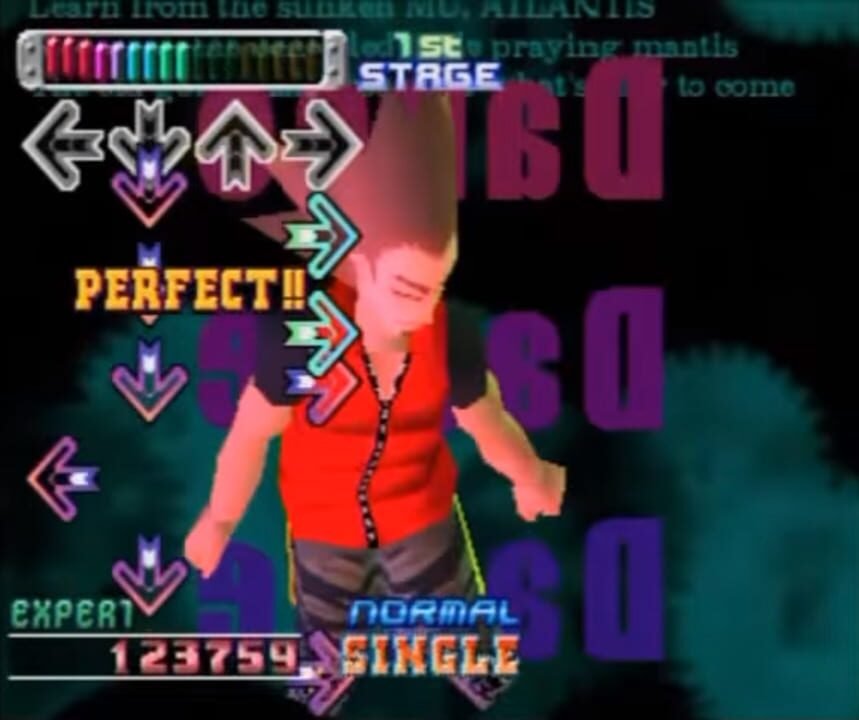
\includegraphics[scale=0.2]{obrazki/ddrgameplay.jpg}
    \caption{\textit{Dance Dance Revolution} gameplay, showing previously described gameplay elements such as health bar and hit notes with matching alignment bar -- taking a form of note outline. Music video is shown playing in the background. \cite{ddrgameplay}}
    \label{fig:ddr_gameplay}
\end{figure}
\pagebreak

Taking these games as examples, the core gameplay of all rhythm games is based on performing an action in accordance with the music's rhythm and displayed pattern. It can be defined that a rhythm game is a medium that puts strong emphasis on a player's rhythm sense, coordination, and reflexes. Another staple of the medium is often the presence of a custom controller, as demonstrated by \textit{beatmania} and \textit{Dance Dance Revolution}. This stays true to this day -- BEMANI is still publishing new installments of these franchises as of 2024, as well as other rhythm games that incorporate all aforementioned mechanics. An example of another immensely popular series featuring such would be Activision's \textit{Guitar Hero} series that successfully ported the arcade experience into the living room, bundling the game with the controller starting on the 6th generation of video game consoles. As Andreas Rauscher described in Scoring Play - Soundtracks and Video Game Genres: "The user plays the notes shown on the screen with a special game controller reminiscent of a musical toy. Guitar Hero employs a plastic guitar with five buttons simulating the fret and another button used to imitate the strumming." (Rauscher 2013: 96). \cite{MusicMedien}

\begin{figure}[h]
    \centering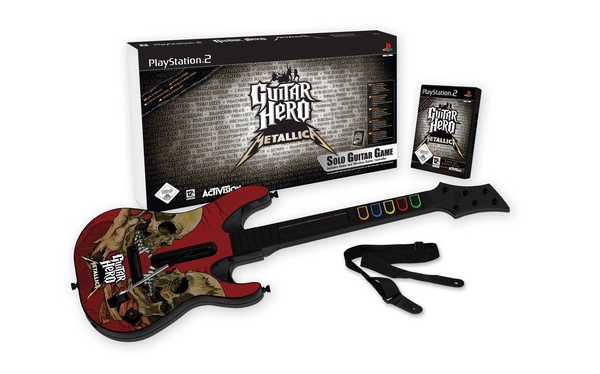
\includegraphics[scale=0.2]{obrazki/gh2bundle.jpg}
    \caption{\textit{Guitar Hero Metallica} PS2 bundle, showing the game disc and plastic guitar controller. \cite{gh2bundle}}
    \label{fig:gh2_bundle}
\end{figure}


The \textit{Guitar Hero} series played crucial part in making rhythm games more popular in the Western regions of the globe, as it featured popular rock and metal songs that attracted new audiences. As Louis-Martin Guay and Dominic Arsenault stated in their chapter of the book \textit{Heavy Metal Generations}: "Heavy metal and video games share an almost simultaneous birth, with Black Sabbath’s debut album in 1970 and Nolan Bushnell’s Computer Space in 1971. Since the birth of these two subcultures in the early seventies, a growing number of interactions between metal music and video games can be observed" (Guay and Arsenault 2012: 1). \cite{heavymetal}. In this chapter, authors are describing the relation between this particular music genre and games such as pinballs, arcades, amusement parks and video games. Because musicians saw games and their soundtracks as an opportunity to promote their music and reach new audiences, many bands have started licensing their music to game franchises. Naturally, as music and songs are a crucial part of rhythm games, this genre has been a perfect fit for such collaborations. Furthermore, as \textit{Guitar Hero} revolves around playing guitar, playing favorite heavy metal songs in this game appears as a natural occurence. Such collaborations have been beneficial for both parties:
\begin{quote}
"Just as music or rhythm video games can host heavy metal, so can heavy metal
host video games. One of the highest-profile examples of this crossover is the
speed power metal band DragonForce, that owes much of its mainstream
popularity to the inclusion of their song \textit{‘Through the Fire and Flames’} on Guitar Hero III: Legends of Rock in 2007. Time and again, DragonForce guitarist HermanLi has cited video games as a major influence" (Guay and Arsenault 2012: 2). \cite{heavymetal}.
\end{quote}
In addition to this mutual benefit between musicians and game developers, the inclusion of songs from real music bands also contributes to the player experience, allowing players to immerse themselves in the game as part of their favorite band. This trope is further reinforced by the Career Mode, the equivalent of the "story mode" in other games. In this gamemode, the player is taking a role of a rockstar, making various performances in order to progress as a musician. Such mode provides a sense of progression and achievement, making the game more engaging and rewarding.

\section{Further developments}
Subsequently, rhythm games were released to both arcades and other platforms, such as home and handheld consoles or PCs. In order to relocate the experience of arcade booths into the home, input devices of arcade games were adapted into home versions of dedicated controllers. For example, an open-source project \textit{StepMania}, which is both a PC game and game engine at the same time, was developed with the purpose of replicating the \textit{Dance Dance Revolution} experience at home. It can be played with keyboard or dance pads matching the pattern of \textit{Dance Dance Revolution}, or alternatively following \textit{Pump It Up!} (Andamiro) controls -- a dance game with 4 buttons placed diagonally and one extra button in the middle.

\begin{figure}[h]
    \centering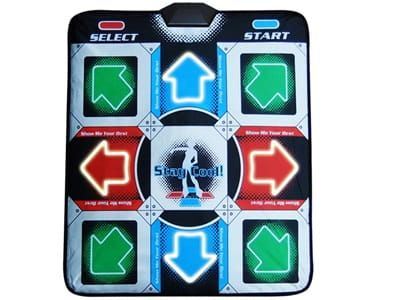
\includegraphics[scale=0.2]{obrazki/ddrsoftpad.jpg}
    \caption{A soft dance-pad which can be used to play both \textit{Dance Dance Revolution} and \textit{Pump it Up!} at home. It can be plugged into a PC or a console. \cite{ddrsoftpad}}
    \label{fig:ddr_softpad}
\end{figure}

In the present day, there are many popular PC games that do not require any dedicated controllers or input devices, making it easier to enter the genre with basic gaming setup. Games such as \textit{StepMania}, \textit{osu!} or \textit{DJMAX} have online scoreboards and online multiplayer modes that bring players together and create lively communities, making the competitive nature a natural part of their gameplay and purpose for players.

\begin{figure}[h]
    \centering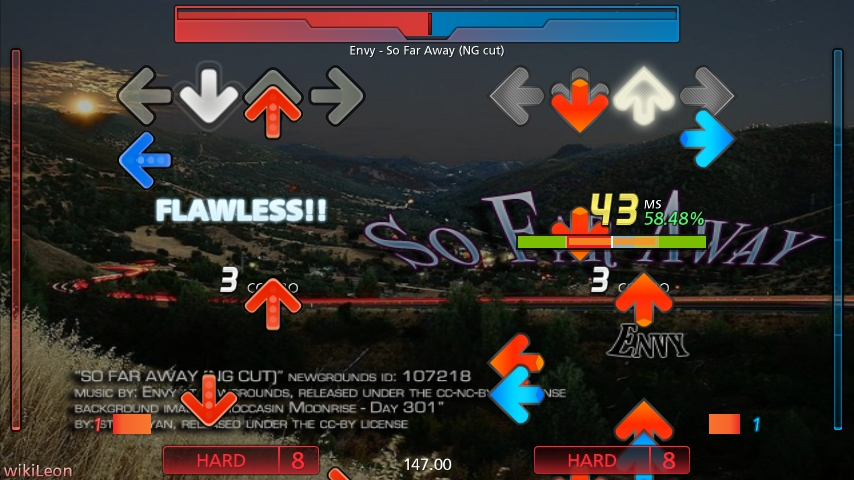
\includegraphics[scale=0.2]{obrazki/sm5multi.jpg}
    \caption{\textit{StepMania} gameplay screenshot, showing Multiplayer Mode where 2 players are competing with each other for better score. \cite{sm5multi}}
    \label{fig:sm5_multi}
\end{figure}
\pagebreak
\begin{figure}[h]
    \centering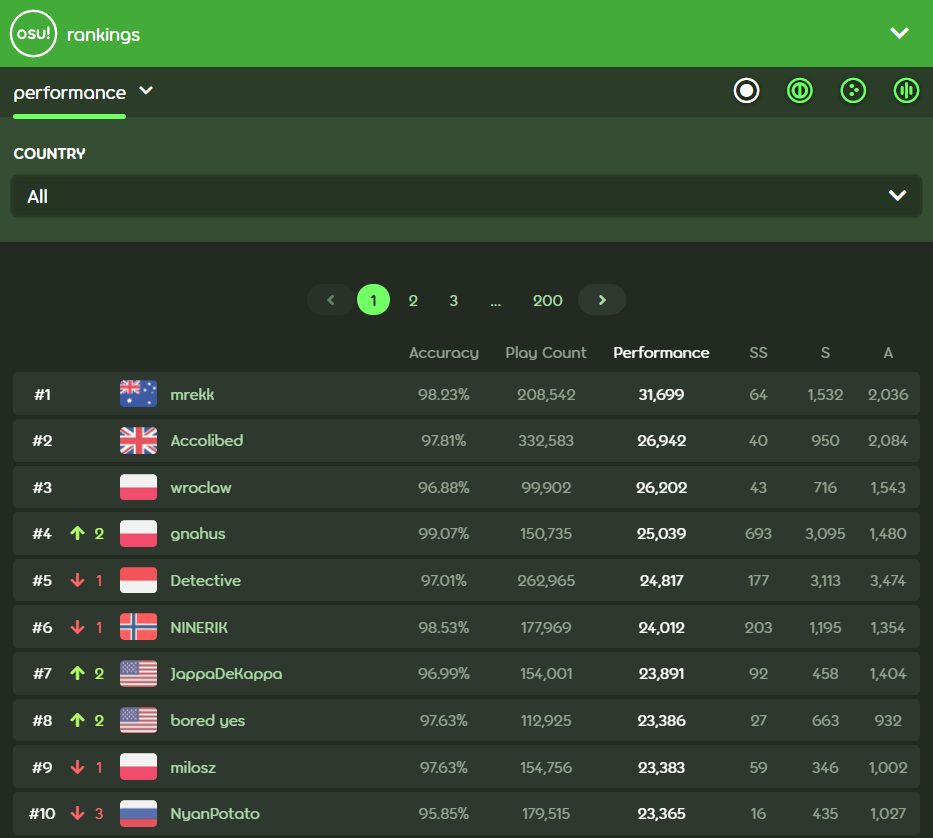
\includegraphics[scale=0.155]{obrazki/osuleaderboards.png}
    \caption{\textit{osu!} online leaderboards as of Jan 2025, showing top players performance from around the world. \cite{osuleaderboards}}
    \label{fig:osu_leaderboards}
\end{figure}
 
On the other hand, there are many arcade games that have unique controllers of various forms. 
One such arcade game that is worth mentioning is \textit{WACCA}, developed and published by Marvelous, which was created in collaboration with HARDCORE TANO*C and released in 2020. The game's user interface is enclosed in a circle, surrounded by a circular, segmented ring panel on the screen edges. The notes appear on the center screen, approaching the player through the ring panels. Because of its fun form somehow resembling a washing machine drum, this game stands out from other rhythm game arcades, as it's financially unviable to port to a home console or PC due to this control scheme and gameplay.

\begin{figure}[h]
    \centering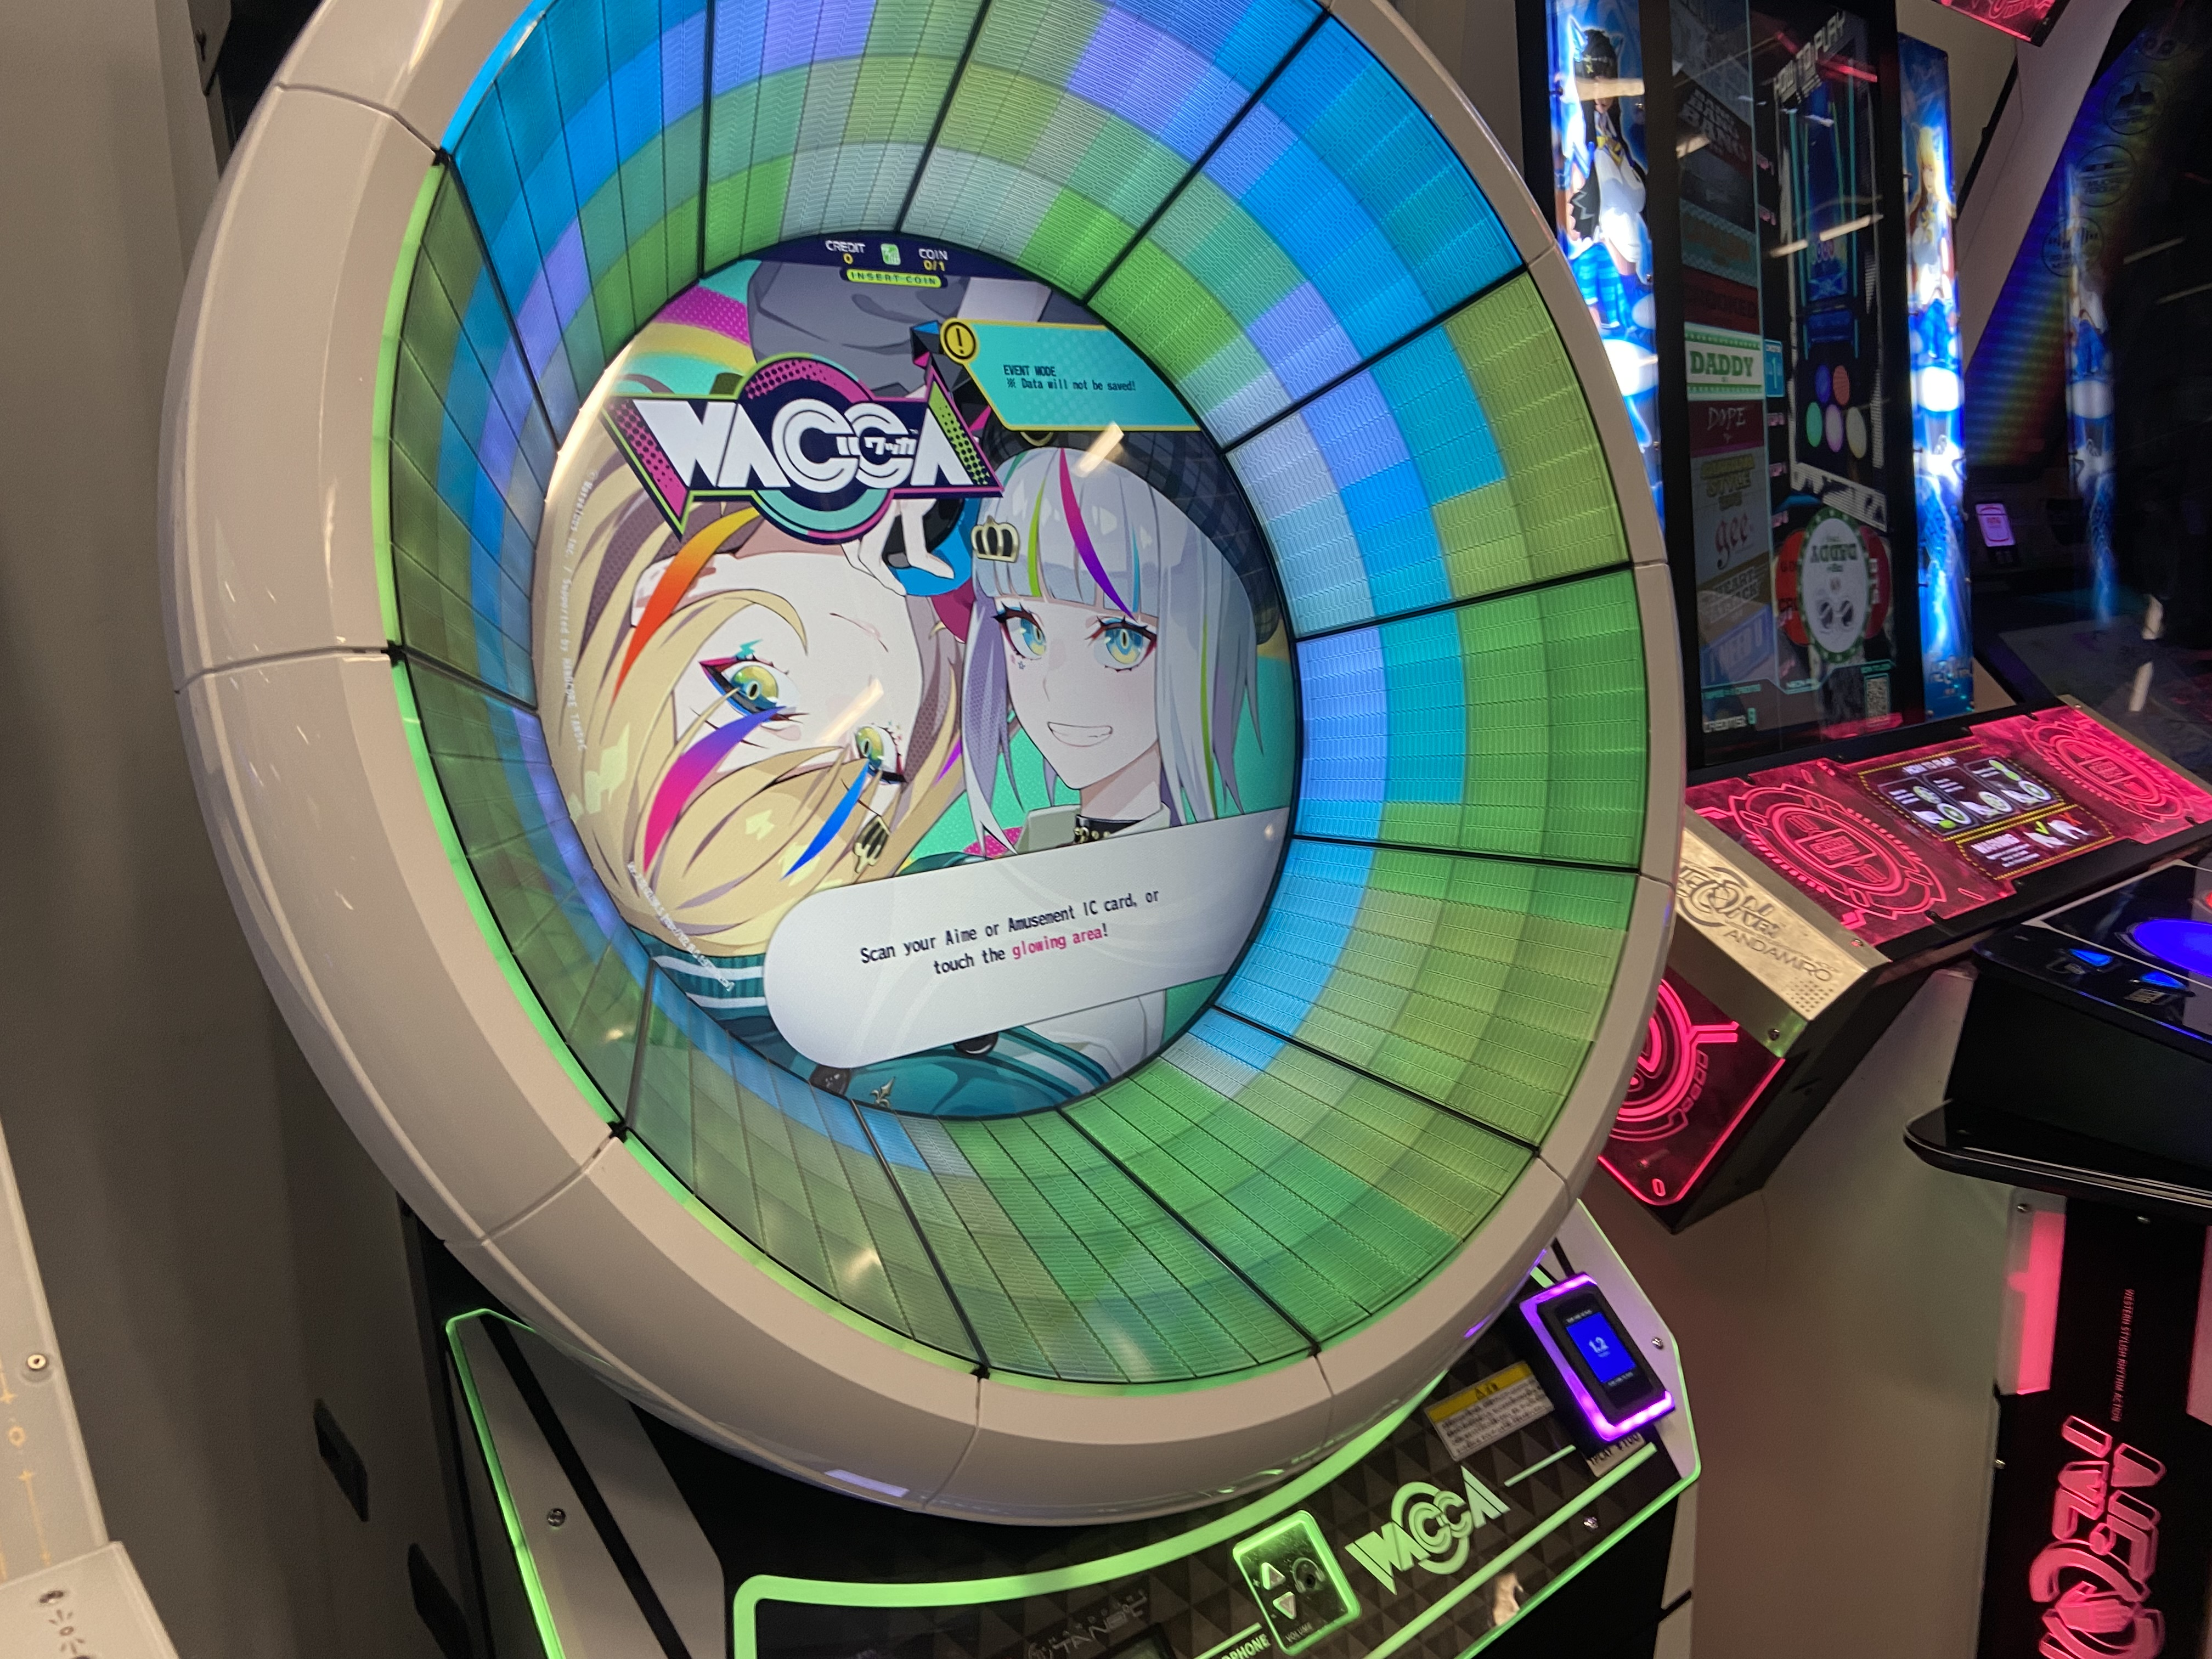
\includegraphics[scale=0.01]{obrazki/waccaarcade.jpg}
    \caption{\textit{WACCA} arcade booth, showing its unique form and controls. \cite{waccaarcade}}
    \label{fig:wacca_arcade}
\end{figure}

The genre of rhythm games also has immense value as an educational tool, as shown through the release of \textit{Rocksmith} by Ubisoft. Instead of using a fake plastic controller, the game allows the player to plug in any real electronic guitar, making it the centerpoint of the game. The game's interface is similar to \textit{Guitar Hero}'s stage, but approaching notes are more specific in order to instruct the player about what grips and strings are supposed to be used. Due to using a real guitar instead of a plastic device, the game was received as a great development milestone in the genre, highlighted by the educational value provided by playing on an actual instrument, as creating a digital rhythm game with real instruments as an input device was a notable achievement for the genre. The game is developed to this day in the form of \textit{Rocksmith+} -- a free-to-play title available on PC, monetized through in-app purchases of songs and lessons.

As Fares Kayali stated in his thesis \textit{Playing Music: Design, Theory, and Practice of Music-based Games} \cite{faresplayingmusic}: 
\begin{quote}
    Overall, rhythm games have changed very little over time. The only changes Harmonix made to the much older Konami games concerned perspective and direct control of the underlying soundtrack. Distinction between rhythm games revolves mostly around the different input devices. From floor mats in DDR, to turntables or guitars, a variety of interfaces have found their way into the homes of rhythm game fans (Kayali 2008: 48).
\end{quote}

Notably, despite the fact that all rhythm games have similar core gameplay, with the development of technology this genre has been able to expand the player experience through the use of new input devices and unique approaches to gameplay. With the rise of technologies such as virtual reality or touch screens, rhythm game developers have utilized new solutions to create new experiences. Because of this, the creativity of game designers is no longer limited as it was in the past.